Intéressons-nous à présent aux phases de traitement de la donnée textuelle, en nous penchant sur la mécanique concrète suivie par le projet \pense. Les sources historiques qui font l’objet des éditions numériques, qu’elles soient conservées par l’\inha ou par ses partenaires le sont généralement sous forme de fonds d’archives, qui doivent donc préalablement être numérisées et transformées par ce biais en format image : il s’agit de les rendre tant lisible sur écran (et ainsi valorisable auprès du public) que traitable par la machine. Au cours de la phase de numérisation, il s’agit de transformer l’objet encore matériel en « données » . Cette transformation « manufacturée » s’accompagne de processus, de traitements qui font l’objet de choix, de réflexions, d’orientation (une médiation soulignée par Johanna Drucker\footcite[p.8]{drucker_is_2013}). 
Après l’étape de la numérisation, viennent les phases d’extraction du texte à partir des images puis d’encodage du texte. Ce sont ces étapes que nous explorerons dans \hyperlink{chap3}{le prochain chapitre}. Nous nous concentrerons ici sur la chaîne de traitement appliquée en vue de l’édition du corpus de correspondance Doucet/René-Jean.

\subsection{De la numérisation à la « mise en données » : la transcription et le balisage, premières étapes de la curation de données}

\subsubsection{Politique de transcription suivie}

\textbfit{Un usage relativement hétérodoxe et assumé de l’outil Transkribus}

Pour traiter les documents manuscrits (entre autres) dans le cadre du projet \pense, l’outil Transkribus a été privilégié. Ce logiciel, développé par l’université d’Innsbruck dans le cadre du projet européen READ (\textit{Recognition and Enrichment of Archival Documents}), constitue une plateforme dédiée à la transcription de textes manuscrits. Proposant un modèle ouvert et participatif, il rassemble une vaste communauté de chercheurs, archivistes, et utilisateurs bénévoles\footcite{carius_plateforme_2020}. Le projet READ, qui a permis de créer cet outil, visait justement à établir une collaboration entre plusieurs domaines de spécialité : des archivistes, des chercheurs en sciences humaines, des informaticiens et des bénévoles\footcite{noauthor_recognition_2015}. Il permet non seulement une transcription manuelle ou automatique (au choix), mais aussi l’entraînement de modèles sur mesure, la recherche dans les transcriptions, un proto-balisage compatible avec la \tei,  l’annotation des documents et l'export dans divers formats. 

Le choix de \pense s’est porté sur Transkribus pour plusieurs raisons. Comme l'explique Sébastien Biay, Transkribus dispose d’un atout majeur en termes d’ergonomie en comparaison avec d’autres outils disponibles, notamment E-Scriptorium, dont l’utilisation s’avère plus complexe et moins aisée à appréhender par des équipes non formées techniquement\footcite[p.24]{biay_chaine_2022}. Son application en ligne (elle-même plus facile d’accès que le client expert bureau en local – comme le note également Jean-Christophe Carius\footcite{carius_plateforme_2020}, ce qui a donné lieu à l’élaboration d’une fiche explicative synthétique pour aider les chercheurs à naviguer dans le modèle de données appliqué par la logique de Transkribus\footcite{inha_schema_nodate}) demeure plus intuitive et plus facile à prendre en main par une équipe non spécialiste d’humanités numériques.  Cette dimension d’accessibilité est un facteur décisif pour le projet \pense, qui vise à impliquer les chercheurs dans l'élaboration de l'édition numérique sans toutefois les forcer à se transformer en développeurs professionnels. Il s'agit de créer un environnement collaboratif où les historiens de l'art peuvent interagir directement avec les outils numériques, tout en restant au cœur du processus de recherche, au lieu d'être isolés des enjeux techniques. 
Signalons qu’à cet effet, des tutoriels\footcite{carius_plateforme_2020} existent en ligne pour familiariser les chercheurs avec l’usage de cet outil\footcite{perrin_tutoriel_2019}.

En ce qui concerne l’export des données, Transkribus permet une extraction en \tei, un format largement utilisé pour l’encodage de textes en humanités numériques francophones. L’utilisateur peut non seulement transcrire, mais aussi baliser le texte, un balisage qui n’est pas complètement rudimentaire (possibilité d’ajouts d’attributs). Avec Transkribus, ce processus est facilité par une interface graphique intuitive, bien plus accessible pour un non-spécialiste qu’une arborescence \xml. Ainsi, les chercheurs peuvent directement baliser des éléments comme des noms de personnes (\textit{persName}), des lieux (\textit{placeName}), ou encore des événements. Un système de balisage, appuyé sur le standard \tei, en cohérence avec le public visé par le service, est proposé, mais une personnalisation demeure possible. Ce balisage s’adapte au contexte des documents étudiés, tout en permettant une personnalisation selon les besoins du projet\footcite{noauthor_pour_nodate}. 
A l’export, on obtient des fichiers \tei à l’architecture simple, en trois parties, comprenant \textbf{<teiHeader>}, \textbf{<facsimile>} et \textbf{<text>}. 

L’ergonomie de Transkribus est également saluée par d'autres projets académiques qui l’ont adopté, comme l'ANR « Foucault Fiches de lecture », où le logiciel a été utilisé pour faciliter la transcription semi-automatique des documents, grâce à une phase d'apprentissage basée sur des réseaux neuronaux (\hyperlink{chap6}{voir chapitre 6}) \footcite[p.104]{bermes_patrimoine_2020}.

Dans le domaine patrimonial, l’utilisation de Transkribus ne se limite pas aux bibliothèques et aux archives, il a aussi trouvé sa place dans les musées. Bien que le recours à la reconnaissance de texte manuscrit (\htr) reste discret dans ce milieu, comme le souligne Alix Chagué, Transkribus a joué un rôle déterminant dans son appropriation par des institutions culturelles : en effet, la quasi-totalité des musées ayant eu recours à l’\htr se sont appuyés sur le logiciel, apprécié pour permettre aux utilisateurs de maîtriser chaque étape de la chaîne de traitement, de la numérisation à l’obtention d’une extraction textuelle, et de « gérer de manière autonome leurs campagnes de transcription » \footcite[p.4]{chague_intelligence_2022}. Transkribus est apprécié en ce qu’il permet de manière ergonomique et relativement transparente pour l’utilisateur d’entraîner des modèles d’IA pour la reconnaissance optique de caractères manuscrits ou typographiés en les affinant (\textit{fine-tuning}) par des vérités terrains (\textit{ground truth}), échantillons représentatifs restreint du corpus étudié mais suffisamment important pour que le modèle puisse assimiler les motifs récurrents.
Cependant, il faut noter dans le cadre du projet \pense, cet aspect n’a pas été pleinement exploité. En effet, le projet a plutôt fait le choix de la transcription manuelle, en raison notamment de la complexité des documents traités, comme nous le verrons plus loin. 
Cette décision a été motivée par plusieurs facteurs : l’hétérogénéité des manuscrits (présence de plusieurs scripteurs pour des projets comme celui de Barye, ou mise en page irrégulière comme dans le cas de Doucet), ou encore la faible volumétrie des documents dans le cas de fonds comme celui de Doucet, insuffisante pour constituer un ensemble représentatif pour l'apprentissage d’un modèle\footcite{carius_plateforme_2020}. Si la segmentation automatique (également proposée par Transkribus) a été explorée notamment dans le cas du projet Thierry, qui semble présenter une relative régularité de mise en page, la tâche de transcription demeure manuelle, pour des raisons évoquées notamment \hyperlink{chap1}{dans le précédent chapitre} (présence de caractères non latins, abréviations non développées, ajouts manuscrits et graphies de lieux parfois non répertoriées – translittérations non fixées depuis le cyrillique ou l’alphabet arménien notamment). Nous aborderons plus en détail les raisons du choix de la transcription manuelle dans le \hyperlink{chap4}{chapitre 4}.
\newline
\textbfit{De l’importance de l’établissement d’une politique de transcription en amont}\\

Le projet d’édition numérique \pense s’est rapidement confronté à une problématique récurrente dans ce type de travail : celle de la cohérence du balisage, une difficulté qu’il aurait été possible d’éviter par une réflexion approfondie sur la transcription en amont. Comme l’indiquent Peter Robinson et Gautier Poupeau\footnote{Dans \footcite{poupeau_reflexions_2004} et \footcite{poupeau_ledition_2008}}, l’élaboration d’une politique de balisage explicite, partagée entre les chercheurs et les ingénieurs, est une étape fondamentale à mener en amont pour s’assurer de la cohérence du travail éditorial. Robinson, de son côté, insiste sur la nécessité de fonder toute édition numérique sur une politique de transcription claire et basée sur des principes explicites\footcite{blanc_feracci_quest-ce_2022}. 
Une telle anticipation aurait pu permettre de résoudre des difficultés spécifiques, notamment celle de l’application irrégulière de balises comme \textbf{`<orgName>`} et \textbf{`<work>`}, qui, dans certaines portions du corpus, sont présentes de manière inégale. Ce manque de constance dans le balisage se révèle particulièrement problématique lors du traitement automatisé des données textuelles, perturbant ainsi l’identification correcte des entités.
L’exemple du projet Thierry, où une réflexion sur le balisage est menée dès le départ, met en lumière l’importance de ce travail préparatoire, non seulement pour éviter des incohérences, mais aussi pour permettre l’intégration des exigences des chercheurs avec celles des ingénieurs. En effet, cette approche concertée favorise une meilleure harmonisation des besoins en termes de contenu scientifique et de traitement numérique, garantissant une plus grande efficacité dans la gestion des données. Cette différence d’approche entre les projets Doucet et Thierry peut en partie s’expliquer par la plus grande maturité de \pense dont bénéficie le projet Thierry, qui a débuté en 2023, à la différence du projet Doucet, qui a vu la phase de transcription et de balisage débuter bien plus tôt, à une époque où l’expérience de \pense avec Transkribus comme avec le standard \tei était peut-être moins importante.
\newline
\textbfit{Projet d’enrichissement non abouti}\\

Un projet d’enrichissement des éléments propres à la correspondance, inspiré des propositions faites dans le manuel \textit{Encoding Correspondence}\footcite{dumont_encoding_2019}, élaboré par le \tei Special Interest Group on Correspondence, et mettant en avant une série de balises TEI spécifiques adaptées à la structure et aux conventions des échanges épistolaires occidentaux, n’a pu par exemple être mené à son terme. Parmi les objectifs initialement envisagés, il était question d’ajouter des balises jugées manquantes dans le <body>, le corps du texte, parmi lesquelles : 

\begin{itemize}[label=\textbullet]
    \item \textbf{<pb/>} (\textit{page beginning}), accompagné de l’attribut @type ayant en valeur ‘folio’ : ceci afin de baliser le marquage de l’information typographique présente sur certaines lettres (dans le sous-ensemble NAF13124), dont l’origine n’est pas pleinement connue, mais qui permet de constituer, dans une approche « génétique » du fonds, un premier marqueur de la logique de classement appliquée soit par René-Jean, soit par la BnF qui a reçu la majeure partie du fonds en 1946.  

    \begin{figure}[h] 
        \centering 
        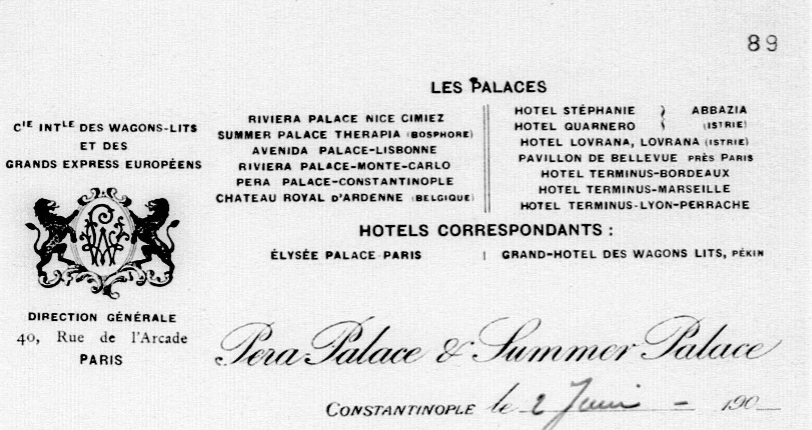
\includegraphics[width=0.8\textwidth]{folio_doucet} 
        \caption{Copie de la lettre bnf\_naf13124\_2\_62, portant la mention typographiée du « folio », « 89 » dans l’angle supérieur droit.} 
        \label{fig:doucet-folio} 
    \end{figure}

    Un autre élément de type « foliotation » manuscrit celui-là et qui n’est ni de la main de Jacques Doucet ni de la main de René-Jean, est présent dans le corpus (sous-ensemble « Autographe 143-145 ») et pourrait faire l’objet d’un balisage similaire (avec quelques variations notamment dans la valeur de l’attribut, qui serait à déterminer auprès de la responsable scientifique). Il s’agit d’une numérotation a priori indépendante de la foliotation, vraisemblablement rajoutée lors de l’archivage du corpus, possiblement par Sylvie Maignan, la fille de René-Jean, qui a effectué elle-même un classement et une numérotation des feuillets du corpus avant d’en faire don à la Bibliothèque de l’\inha au début des années 2000. 

    \begin{figure}[h] 
        \centering 
        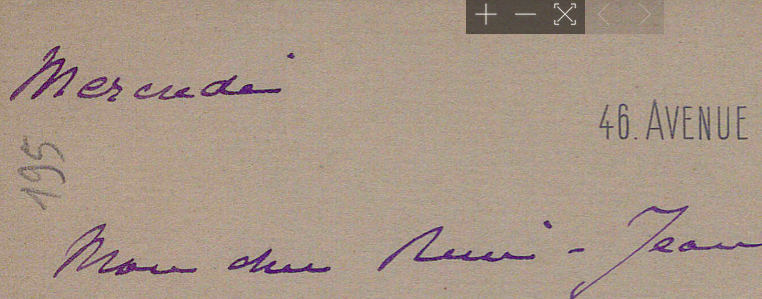
\includegraphics[width=0.8\textwidth]{numerotation_maignan} 
        \caption{Copie de la lettre BINHA, Aut. 143\_02\_195, portant la mention manuscrite de la numérotation appliquée par Sylvie Maignan, « 195 » au crayon à papier, perpendiculaire par rapport au sens de l’écriture, flanc gauche.} 
        \label{fig:doucet-maignan} 
    \end{figure}

    Lors de la transcription manuelle de la correspondance, le choix a été de marquer l’existence de ces ajouts directement dans le corps du texte, en s’inscrivant ainsi dans des choix de transcription propres à l’édition traditionnelle : l’italique et l’usage de parenthèses ont ainsi été privilégiées. Ce choix, pertinent dans le cadre d’une édition papier ou traditionnelle, n’intégrant pas l’usage d’un format balisé, peut être limitant dans le cas d’une édition \tei, en ce qu’il confond sémantique et typographie. 
    En \tei, l’information peut être rendue par le choix de balises appropriées, qui, dans un deuxième temps, lors de la phase de transformation vers l’\html, peut se traduire par des variations typographiques. L’intégration d’informations « périphériques » au texte d’origine directement dans le corps du texte peut en effet apparaître gênante lors du traitement automatique, d’où cette initiale orientation vers le choix de balise \textbf{<pb/>}, recommandée par le manuel \textit{Encoding Correspondence}. 
    \item L’usage de la balise \textbf{<add/>} comprenant l’attribut @hand et la valeur ‘RJ’ (pour René-Jean), aurait également pu permettre de baliser les passages de texte ajoutés postérieurement par René-Jean et ainsi éviter, de façon analogue au cas cité ci-dessus, l’ajout par l’éditeur du texte brut « (de la main de René-Jean) » en italique. 
    \item \textbf{<back/>} pour les informations textuelles propre à l’agencement des cartes postales (description de la carte postale située au dos de la zone de texte).
    \item \textbf{<fw/>} (\textit{form work}) accompagné de l’attribut @type et de la valeur ‘header’ pour les en-têtes de papiers à en-têtes, comme les documents portant le nom et l’adresse de l’hôtel où séjourne Doucet par exemple – cas fréquemment rencontré dans le corpus.
    \item \textbf{<stamp/>} ou \textbf{<figure @type=’cachet’/>} pour l’encodage des informations relatives aux éléments textuels rattachés à des timbres ou des tampons.
    \item L’usage de balises telles que \textbf{<signed/>} pour la signature, \textbf{<salute/>} pour la formule de politesse ou encore \textbf{<dateline/>} pour les informations de datation aurait également pu être pertinent. 
\end{itemize}

L’irrégularité de placement , vis-à-vis de ces balises, des parties textuelles qui auraient pu faire l’objet d’un balisage tel que décrit plus haut, combiné à la grande variation de ce type d’information, complique encore un peu plus leur identification et leur repérage. 
Une balise de description spécifique aux échange épistolaires dans le \textbf{<teiHeader/>} était également envisageable, il s’agit de la balise \textbf{<correspDesc/>} incluse dans le \textbf{<profileDesc/>}\footcite{tei_consortium_tei_2024}, permettant d’encoder précisément les informations relatives à chaque acteur de la correspondance, pour chaque lettre échangée.

Plusieurs obstacles ont entravé la mise en œuvre de ces enrichissements. 
D’une part, l’export \tei de la transcription manuelle obtenu via l’outil Transkribus a généré un grand nombre de balises auto-fermantes, telles que \textbf{`<lb/>`}, \textbf{`<ab/>`}, \textbf{`<pb/>`}, ou \textbf{`<fw/>`}, utilisées pour signaler la correspondance entre le texte et l’image ou pour marquer les éléments de mise en page, qui ont pu gêner la circulation dans l’arborescence \xml. Ces balises, bien qu’utiles pour la structuration visuelle du texte, se sont parfois avérées problématiques du point de vue de la préservation de la logique sémantique du balisage textuel. 
En particulier, la balise \textbf{`<lb/>`}, indiquant le passage à la ligne (\textit{line beginning}), a provoqué des coupures gênantes dans certaines balises, comme les noms de personnes. Par exemple, un nom complet écrit sur deux lignes se retrouve scindé en deux balises `<persName>`, compliquant ainsi le traitement automatique de ces données nominatives. Cet effet est exacerbé lorsque les parties textuelles concernées ne sont pas homogènes ou apparaissent de manière irrégulière, rendant plus complexe leur balisage et leur repérage ultérieur. En effet, dans une situation telle que « Jacques » apparaît en fin de ligne et « Doucet » en début de ligne suivante, le résultat suivant est susceptible de se produire : 
\begin{minted}[linenos,frame=lines,fontsize=\small]{xml}
    <persName>Jacques</persName>
    <lb/>
    <persName>Doucet</persName>
\end{minted}, provoquant, lors de l’indexation automatique, l’identification de deux entités nommées pour une seule personne. 

Les balises encapsulées, comme \textbf{`<persName>`} dans un \textbf{`<choice>`}, constituent une autre source de complications. Dans certains cas, ces balises n’ont pas été correctement identifiées par les outils de repérage utilisés, comme en témoigne l’exemple du nom « Holleau » dans le fichier bnf\_naf13124\_2\_60, où la balise \textbf{`<sic>`} (portant la valeur de l’adverbe « sic », signalant une graphie (ici de nom propre), jugée irrégulière), englobant le nom pose un problème pour certains outils de repérage des balises, du fait d’espaces surnuméraires induits par la présence d’autres balises au sein de la balise \textbf{<persName>} :
    \begin{minted}[linenos,frame=lines,fontsize=\small]{xml} 
    <persName>
        <comment>
            <choice>
                <corr/>
                <sic>Holleau</sic>
            </choice>
        </comment>
    </persName>
    \end{minted}.
\newline
\textbfit{Un héritage parfois problématique de l’édition traditionnelle}

Les difficultés rencontrées dans le projet \pense trouvent également leurs racines dans un héritage parfois pesant ou inadapté de l’édition traditionnelle, où les conventions typographiques priment souvent sur les potentialités offertes par l’édition numérique. En effet, dans certaines parties du corpus, le choix a été fait de suivre les conventions de l’édition papier, introduisant des mentions comme « (de la main de René-Jean) » directement dans le texte, en italique et entre parenthèses. Cette décision, motivée par la volonté de rester fidèle aux conventions éditoriales classiques\footcite{nougaret_ledition_2015}, a cependant posé problème dans le cadre de l’édition numérique, comme nous l’avons brièvement évoqué plus haut. 
Cette approche peut ainsi être jugée comme ne prenant pas toujours en compte les spécificités de l’édition numérique et notamment les potentialités du balisage, en confondant mise en forme finale et traitement intermédiaire du corpus : là où il serait possible d’utiliser une balise \tei sémantiquement appropriée et qui serait éventuellement restituée par une traduction typographique  respectant les conventions de l’édition classique (italique, parenthèses, mention complémentaire…), le choix a été fait d’intégrer directement dans le texte du corpus une indication éditoriale, brouillant potentiellement les lignes entre texte original et texte édité, une situation susceptible de poser problème dans le cas d’une édition qui se veut « diplomatique ».

En effet, la volonté affirmée de proposer une double lecture, à la fois diplomatique (imitative) et critique (proposant un apparat critique et une révision du texte) au lecteur\footnote{« Tout le sens du projet \pense est donc de restituer cette épaisseur du texte manuscrit, tout en donnant accès à une version éditorialisée que l’internaute pourra à loisir citer et commenter à son tour », dans \footcite[p.2]{carius_principes_2024}}, vient ainsi se heurter aux potentialités du numérique, car on peut voir dans ces complexités de balisage un mélange entre plusieurs formes éditoriales, notamment dans l’exemple de la note « de la main de RJ » : le fait d’inclure dans le texte cette mention de l’éditeur, distinguée du corps du texte par un simple marquage typographique comme des crochets ou des parenthèses, est à mettre en lien avec un réflexe éditorial critique traditionnel, et vient gêner l’édition diplomatique au sens strict (dans lequel elle n’a pas lieu d’être). 
Il est peut-être également possible de voir dans la préférence pour un balisage typographique (tel qu’avec la balise de mise en forme \textbf{<hi/>}) au détriment du balisage sémantique (\textbf{<add @hand/>}) une certaine hâte à produire une version finale du texte, sans avoir pleinement exploré les potentialités de la réflexion numérique. 

\subsubsection{Choix de balisage des textes}
\newline
\textbfit{Le standard TEI}\\

Le projet \tei se présente comme une entreprise « durable et influente » dans le domaine des humanités numériques. Conçu à la fin des années 1980 autour de l’élaboration d’une « grammaire » du langage \sgml puis \xml adaptée à l’encodage de documents patrimoniaux, il affiche pour ambition d’offrir un cadre clair, adaptable et facilement implémentable pour normaliser et  structurer la production de données textuelles, essentiellement destinées à la recherche en \shs. Comme le souligne Lou Burnard, l’un des fondateurs de l’initiative, la \tei émet des recommandations pour la création de textes numériques, en portant l’ambition de cultiver la collaboration au sein d’une vaste communauté scientifique (appuyée sur son Consortium, rassemblement d’organisations partenaires pour la plupart issues du monde universitaire)\footcite{burnard_quest-ce_2015}. 
Ces recommandations mettent particulièrement l'accent sur l'analyse sémantique du texte et garantissent une interopérabilité avec différents environnements logiciels permettant la réutilisation des données, car elles se veulent indépendantes de tout cadre technique spécifique. Le standard a connu plusieurs évolutions depuis sa première version en 1987, et la cinquième édition (P5), publiée en 2007, étant désormais fondée exclusivement sur \xml, abandonnant ainsi le \sgml utilisé dans les premières versions.
La flexibilité de la \tei permet des personnalisations étendues grâce au principe de l’\odd, qui autorise la création de schémas d’encodage adaptés à des projets spécifiques\footcite{noauthor_odd_nodate}.

Les recommandations proposées par la \tei sont compilées dans un document unique appelé \textit{Guidelines}, décrivant en détail (sous la forme de l’ODD originelle de la version P5) les bonnes pratiques pour l’encodage des textes numériques. 

Un document encodé en \tei est structuré en plusieurs sections essentielles. La première balise croisée dans l’arborescence \xml d’un texte encodé en \tei est le \textbf{`<teiHeader/>`}, qui contient l’ensemble des métadonnées du fichier (titre, nom de l’auteur, contexte de production, etc.). Cette balise se compose généralement de quatre sections principales, dont une seule est obligatoire\footcite{tei_consortium_tei_2023} : le \textbf{`<fileDesc/>`}, qui décrit les aspects bibliographiques du document électronique. Parmi les trois autres sections généralement retrouvées, citons la balise \textbf{`<encodingDesc/>`} qui documente « la relation entre le texte numérique et ses sources », à savoir, le plus souvent, la politique d’encodage adoptée ; le \textbf{`<profileDesc/>`} qui fournit des informations sur les « aspects non bibliographiques » du texte ; enfin, le \textbf{`<revisionDesc/>`} résume l’historique des modifications apportées au fichier depuis sa création, à la manière d’un fichier \textit{log}. 

La structure des documents \tei se prolonge avec la balise \textbf{`<text/>`}, qui renferme la transcription du texte divisé en plusieurs sections : \textbf{`<front/>`} pour les éléments préliminaires comme la page de titre, \textbf{`<body/>`} pour le corps principal du texte, et \textbf{`<back/>`} pour les éléments post-liminaires. 
Dans le cadre des documents générés via Transkribus par exemple, une autre balise est systématiquement introduite avant le \textbf{<text/>} : \textbf{`<facsimile/>`}, qui assure un lien entre les fac-similés des documents numérisés et leur transcription en identifiant (grâce à des balises et attributs enfants) par des points « géographiques » l’emplacement du texte (obtenu grâce à la transcription, manuelle ou automatique) au sein de l’image. 

L’usage du standard \tei n’est pas restreint à la seule recherche universitaire, bien que celle-ci demeure son domaine de prédilection. Selon des données recueillies dans le \textit{Digital Catalogue of Digital Editions}, 196 des 337 éditions répertoriées utilisent \xml-\tei comme format d’encodage\footcite{ucl_centre_for_digital_humanities_digital_nodate}. 
Cependant, il existe des cas où des projets préfèrent ne pas utiliser la \tei, comme le souligne Patrick Sahle. Deux raisons principales entrent en jeu pour expliquer ce choix : 
\begin{itemize}
    \item d’une part, l’apprentissage de la \tei peut être perçu comme chronophage, et certains projets estiment ne pas avoir les ressources nécessaires pour maîtriser ces compétences en temps limité, 
    \item d’autre part, des balises \xml personnalisées peuvent mieux correspondre aux spécificités des textes sources que celles proposées par la \tei, offrant une flexibilité supplémentaire\footcite[p.174-75]{sahle_what_2016}.
\end{itemize}
De plus, il est à remarquer que l’encodage en \tei, pour des raisons de compatibilité de caractères, est davantage adapté pour les langues à alphabet latin comme le français, l’anglais ou le latin, tandis que les langues disposant d’un alphabet non-latin ou d’un système d’écriture différent, tels que le cyrillique, l’abjad arabe ou les sinogrammes, rencontrent encore des difficultés d’implémentation dans ce format\footcite[p.177]{sahle_what_2016}.

En France, l’utilisation de la \tei (assez largement partagé dans les projets d’éditions numériques), est plutôt encouragé dans le cadre des projets soutenus par des grandes institutions de recherche. Comme le note \citeauthor{chateau-dutier_editions_2021}, le \textit{Guide des bonnes pratiques numériques} de 2009, rédigé par le Très Grand Équipement Adonis, devenu Huma-Num, recommande explicitement le recours à cette norme pour l’encodage de documents dans le cadre de projets de recherche en \shs\footcite{tge-adonis_guide_2009}. Château-Dutier remarque par ailleurs que l’adoption de la \tei par le milieu de la recherche française, demeure relativement récent : le premier projet français à avoir utilisé la \tei ayant été l’édition des cours d’Antoine Desgodets en 2008\footcite[p.81]{chateau-dutier_editions_2021}. Aujourd’hui, la \tei est devenue un standard largement adopté pour les éditions critiques numériques dans la sphère des humanités numériques francophones\footcite{blanc_feracci_quest-ce_2022}, et notamment en histoire de l’art\footcite[p.82]{chateau-dutier_editions_2021}.
\newline
\textbfit{Les libertés prises par le projet \pense vis-à-vis du standard TEI}\\

Le projet \pense, bien qu’aligné sur le standard \tei, a pris certaines libertés vis-à-vis des recommandations officielles. Il est important ici d’introduire les notions de « conformité » et de « validité » : si, dans le contexte étudié dans ce chapitre, la \textbf{conformité} (ou le caractère « bien formé » d’un document) se réfère au respect de la syntaxe \xml (garanti par exemple par la présence d’une déclaration \xml avant la racine du document, par le respect du principe de non-chevauchement des balises et de l’architecture arborescente propre à \xml, par exemple) ; la \textbf{validité}, elle, concerne le respect de la grammaire particulière, ou du schéma, appliqué au \xml – ici, il s’agit du respect de la « grammaire » \tei : à savoir, le respect de la logique de balisage introduite par \tei : certaines balises ne peuvent être enfants d’autres balises par exemple. Un document conforme peut donc être invalide. 
Le caractère invalide d’un document peut entraîner des problèmes d’interopérabilité, notamment lorsqu’il s’agit d’appliquer des traitements automatiques sur le fichier, nécessitant ainsi un pré-traitement supplémentaire. 

Un exemple concret des choix inhabituels réalisés par le projet \pense concerne l’utilisation d’identifiants non uniques (@xml:id). En effet, l’attribut @xml:id, ayant pour rôle de donner un identifiant unique à des entités déterminées (comme des noms de personnes avec <persName/> ou des noms de lieux, avec <placeName/> par exemple), ne peut avoir qu’une valeur unique dans tout le document encodé\footcite{marsh_xmlid_2005}. Or, lors de la mise en place de l’édition Doucet-René-Jean et de la mise en place de l’identification, cette règle n’a pas été complètement respectée.  Une solution possible pour corriger cette situation est d’intégrer un index des personnes dans la balise \textbf{`<profileDesc>`}, définissant ainsi chaque identifiant unique une fois pour chaque document et permettant de référencer ces identifiants dans le \textbf{`<body>`} du document à l’aide de l’attribut @ref accompagnée d’une valeur identique à la valeur de @xml:id mais précédée d’un croisillon (« # »). 
Bien que cette méthode permette de se conformer tant aux \textit{Guidelines} \tei qu’aux bonnes pratiques d’encodage \xml, sa mise en œuvre est susceptible de s’avérer chronophage. 
L’autre alternative, déjà pratiquée par \pense dans le cadre de l’édition \textit{Barye}, consiste à ne pas utiliser l’attribut @xml:id, mais de lui préférer l’attribut @ref accompagné d’une spécification quant au référentiel utilisé pour formuler l’identifiant (comme @ref-agorha, @ref-idref ou @ref-wikidata). 

Par ailleurs, la question de l’utilisation d’une \odd dans le cadre de \pense mérite d’être posée. L’ODD permet de créer un schéma de validation personnalisé pour une édition numérique au format \tei. Comme le souligne \citeauthor{biay_chaine_2022}, certains projets nécessitent un degré de précision et de spécificité tel qu’il devient nécessaire de produire une ODD\footcite[p.72]{biay_chaine_2022}, mais cela ne semble pas être le cas pour le projet \pense. Étant donné la diversité de nature des projets d’édition numérique, la création d’une \odd n’apparaît pas comme une priorité pour \pense, même si cette option pourrait être envisagée si l’encodage devait devenir plus complexe à l’avenir.

\subsection{L’encodage des métadonnées : transformations appliquées aux en-têtes TEI}

\subsubsection{Enrichissement des métadonnées}

Les transformations appliquées aux fichiers \tei du projet \pense ont permis d’enrichir les métadonnées. Pour réaliser ces modifications, des technologies telles que XQuery et XPath, correspondant aux spécifications du \wwwc, ont été utilisées. Ces langages sont particulièrement adaptés à la manipulation de données en \xml-\tei, car ils permettent de naviguer efficacement dans l’arborescence des fichiers, en passant aisément d’un élément parent à ses éléments enfants. Comme le rappelle Anderson, XQuery est compact, concis et relativement facile à apprendre, ce qui en fait a priori un outil de choix pour les humanistes numériques\footcite{anderson_teaching_nodate}. 
Langage installé sur le Web depuis plus de vingt ans, sa longévité constitue également paradoxalement sa limite fondamentale, en ce que la documentation disponible tend à être ancienne et rattachée à des environnements obsolètes (bien que le langage lui-même n’ait pas grandement évolué depuis la publication de la documentation).  En plus de faciliter les transformations, l’interface de BaseX, utilisée dans le projet, permet de réinjecter directement les modifications dans la base de données.
XQuery s’est révélé particulièrement utile pour l’ajout d’informations manquantes aux fichiers \tei générés par Transkribus, pour la normalisation des données, ainsi que pour l’insertion d’identifiants pérennes à certains éléments.

Le choix des ajouts à opérer pour l’encodage des métadonnées s’est inspiré d’autres projets ayant utilisé la \tei comme le \textit{Thomas Gray Archive}, dont la structure \tei choisie propose une présentation relativement riche des métadonnées\footnote{Voir par exemple le fichier suivant : https://www.thomasgray.org/texts/poems/txt_GrayTh1716_wdeho.xml}.

Les fichiers sur lesquels nous avons travaillé étant directement issus de l’export \tei produit à partir de la transcription Transkribus, l’encodage du \textbf{<teiHeader/>} était particulièrement rudimentaire, ne comprenant que le titre (pour lequel la convention de nommage lors de la transcription avait privilégié l’indication de la cote avant la présentation du contenu), la date lorsqu’elle avait été précisée par l’opérateur effectuant la transcription, ainsi que le nom de l’institution porteuse du projet, la cote, la typologie documentaire, le nombre de page et la langue. 
Nous avons donc choisi d’effectuer les ajouts et transformations suivants, grâce à un script XSLT encapsulé dans un script XQuery  :

\begin{itemize}[label=\textbullet]
    \item \textbf{<projectDesc/>} et \textbf{<editorialDesc/>} à partir de l’exemple proposé par \textit{The Thomas Gray Archive}
    \item normalisation et suppression des cotes dans les titres
    \item ajout d’un identifiant pérenne (IDREF ou AGORHA) pour les noms d’auteurs, grâce à un attribut @ref
    \item ajout d’un identifiant pérenne \ark de la \bnf dans le \textbf{<seriesStmt/>} pour les documents issus du fonds conservé à la BnF
    \item indication du nom de la responsable scientifique du projet dans le \textbf{<respStmt/>}
    \item normalisation des URL (suppression des espaces et des virgules, susceptibles de gêner le traitement automatique du corpus). 
\end{itemize}[label=\textbullet]

\subsubsection{Préparation en amont d’une fonctionnalité d’interface}

La chercheuse en charge du volet scientifique du projet, Marie-Anne Sarda, a émis le souhait d’une interface finale qui puisse permettre de naviguer aisément entre les différentes collections de la \baa de Jacques Doucet. 
Ce désir s'appuyait sur une typologie d'objets d'art mentionnés dans la correspondance de Doucet, parmi les objets classifiés à l'aide de la balise \textbf{`<work>`}. La fonctionnalité  devrait reposer sur une présentation visuelle de type « cartes \textit{Bootstrap} » des œuvres mentionnées, chaque carte représentant une catégorie d'objets collectionnés par Doucet, comme les estampes, imprimés, photographies ou encore les dessins. En cliquant sur ces cartes, les utilisateurs pourraient accéder à des informations plus détaillées sur les œuvres concernées citées dans la correspondance et, idéalement, les admirer, grâce à de potentiels partenariats avec des institutions de conservation. Cette démarche s'inscrit dans un effort de visualisation visant à permettre aux lecteurs de comprendre concrètement les œuvres dont il est question dans la correspondance de Doucet. Notre travail s’est donc concentré sur la manière d’établir la meilleure façon de préparer en amont, grâce à l’encodage \tei, la future exploitation de cette typologie d’œuvres par les fonctionnalités d’interface. Il s’agissait d’identifier, pour chaque typologie isolée par la chercheuse, les lettres mentionnant des œuvres correspondant à cette typologie, pour permettre à terme leur recherche par facettes.

Pour parvenir à cet objectif, un processus en quatre étapes a été suivi : 
\begin{itemize}
    \item La première a consisté en la création par la chercheuse d'un fichier Excel contenant un alignement entre les lettres individuelles et les typologies d'objets d'art évoqués dans ces lettres.
    \item Ensuite, ce fichier Excel a été transformé en fichier \csv, choisi pour des questions d’interopérabilité, alignant plus clairement les identifiants des lettres avec ceux des typologies.
    \item Dans un troisième temps, un script Python a été utilisé pour modifier les identifiants et les faire coïncider avec ceux présents dans la base de données, en ajoutant une nouvelle colonne dans le \csv.
    \item Enfin, un script XQuery a été employé pour traiter les données du \csv, les transformer en fichier \xml, et enrichir la base de données \tei avec les informations contenues dans ce fichier.
\end{itemize}
   
\subsection{L’encodage du corps du texte}

\subsubsection{Protocole suivi pour l’enrichissement des noms de personnes}

Les noms de personnes, identifiés pour la plupart par la balise \textbf{<persName/>} ne présentaient, à quelques exceptions près (telle que l’usage de la balise @key pour certaines occurrences du nom de Doucet) aucune forme d’enrichissement lors de la reprise des fichiers obtenus par export \tei de la transcription effectuée sur le Transkribus. Il s’agissait donc de permettre une indexation optimale pour les noms de personnes.  

Le processus a débuté à nouveau avec la création d'un fichier Excel de travail par la chercheuse, contenant la forme normalisée (« Nom, Prénom ») du nom des personnes, une courte note biographique, ainsi que leur lieu d'exercice. Ce fichier avait vocation à devenir la source de valeurs pour l’ensemble des attributs choisis pour l’enrichissement : 
\begin{itemize}[label=--]
    \item l’attribut @key présente un format et une graphie normalisée des noms de personnes (« Nom, Prénom »)
    \item l’attribut @xml:id comporte une valeur d’identifiant unique, composée par la première lettre du prénom concaténée au nom de famille entier. Ce choix, apparemment arbitraire, a été cependant motivé par un souci d’intelligibilité du code – il aurait été tout à fait envisageable de choisir un identifiant unique de type \uuid, qui aurait néanmoins souffert d’une certaine opacité. Par ailleurs, la volumétrie de la base traitée étant limitée, la choix d’un tel identifiant n’a pas semblé indispensable.
    \item l’attribut @type indique l’occupation, la profession ou la relation par rapport à Doucet, sur la base des informations fournies par la chercheuse.
    \item l’attribut @subtype désigne ici le lieu d’exercice ou de résidence rattaché à la personne. Cette utilisation diffère légèrement des recommandations \tei\footcite{tei_consortium_tei_nodate}, en ce qu’il ne s’agit pas d’une information d’importance moindre que l’information indiquée dans l’attribut @type, mais d’une donnée indépendante.
    \item l’attribut @ref-agorha fournit quant à lui, lorsque disponible, un lien \ark vers la notice AGORHA de la personne concernée. 
\end{itemize}

Le processus d'enrichissement s'est déroulé en neuf étapes :
\begin{itemize}
    \item La première a consisté en une simplification manuelle du fichier de personnes fourni par la chercheuse.
    \item Un fichier \csv a ensuite été créé pour contenir les variations graphiques des noms de personnes trouvées dans le corpus de correspondances. Pour chaque nom, plusieurs versions graphiques étaient alors alignées (la variation trouvée dans le corpus, la version corrigée et la version dite « unifiée » (sous le format devant être intégré à l’attribut @key)).
    \item Un script Python a alors permis de fusionner les données du fichier d'origine simplifié avec celles du \csv produit précédemment, aboutissant à la création d'un nouveau fichier \csv.
    \item Après quelques modifications manuelles supplémentaires, un autre script Python a réorganisé ce fichier par ordre alphabétique et y a ajouté un numéro d'ordre.
    \item Enfin, un script XQuery a permis de transformer ce \csv en fichier \xml, enrichissant la base de données \tei avec les informations nouvellement obtenues.   
\end{itemize}
